\chapter{Análisis espectrales: resultados numéricos}
\label{chap: resultados numericos analisis espectrales}

Después de todo lo expuesto en las secciones anteriores, tenemos
ya dos alternativas para graficar el espectro
de una señal $x \in \IR^{n}$.

\begin{itemize}
	\item Usando la transformada discreta de Fourier
	(c.f. sección \ref{sec: TDF}), el espectro de
	una señal $x$ es la gráfica de las frecuencias
	enteras dadas (dependiendo de la 
	paridad de $n$) por las
	tablas 6.1 y 6.2
	versus los coeficientes
	$\tau_{n}(x)$ definidos en
	\ref{def: taus}.
	\TODO{Puesto que hacer un análisis con la
	DFT significa expresar a $x$ como una suma
	ponderada de muestreos de senos y cosenos
	de algunas frecuenicas enteras,...}
	
	\item Si, para hacer un análisis espectral, se usan
	las ideas propuestas en 
	la sección
	\ref{sec: metodologia para realizar un analisis espectral que considere frecuencias arbitrarias}, entonces, dado un rango de frecuencias 
	$\omega$,
	el espectro de $x$ es la gráfica de 
	las frecuencias $\omega$ versus	
	los coeficientes
	$\sigma_{n}(x, \omega)$.
	

\TODO{a diferencia de la dft, los casos extremos ya no son
estar o no estar, sino ser perpendicular o ser paralelo a su
representante del espacio monofrecuencial.}
\end{itemize}

Espectro cero: el de TDF
Espectro uno: el de espacios monofrecuenciales

\begin{figure}[H]
	\sidecaption{
	Ejemplo de los espectros resultantes
	de los dos métodos de análisis.
	\label{fig: espectro 1 }
	}
	\centering
	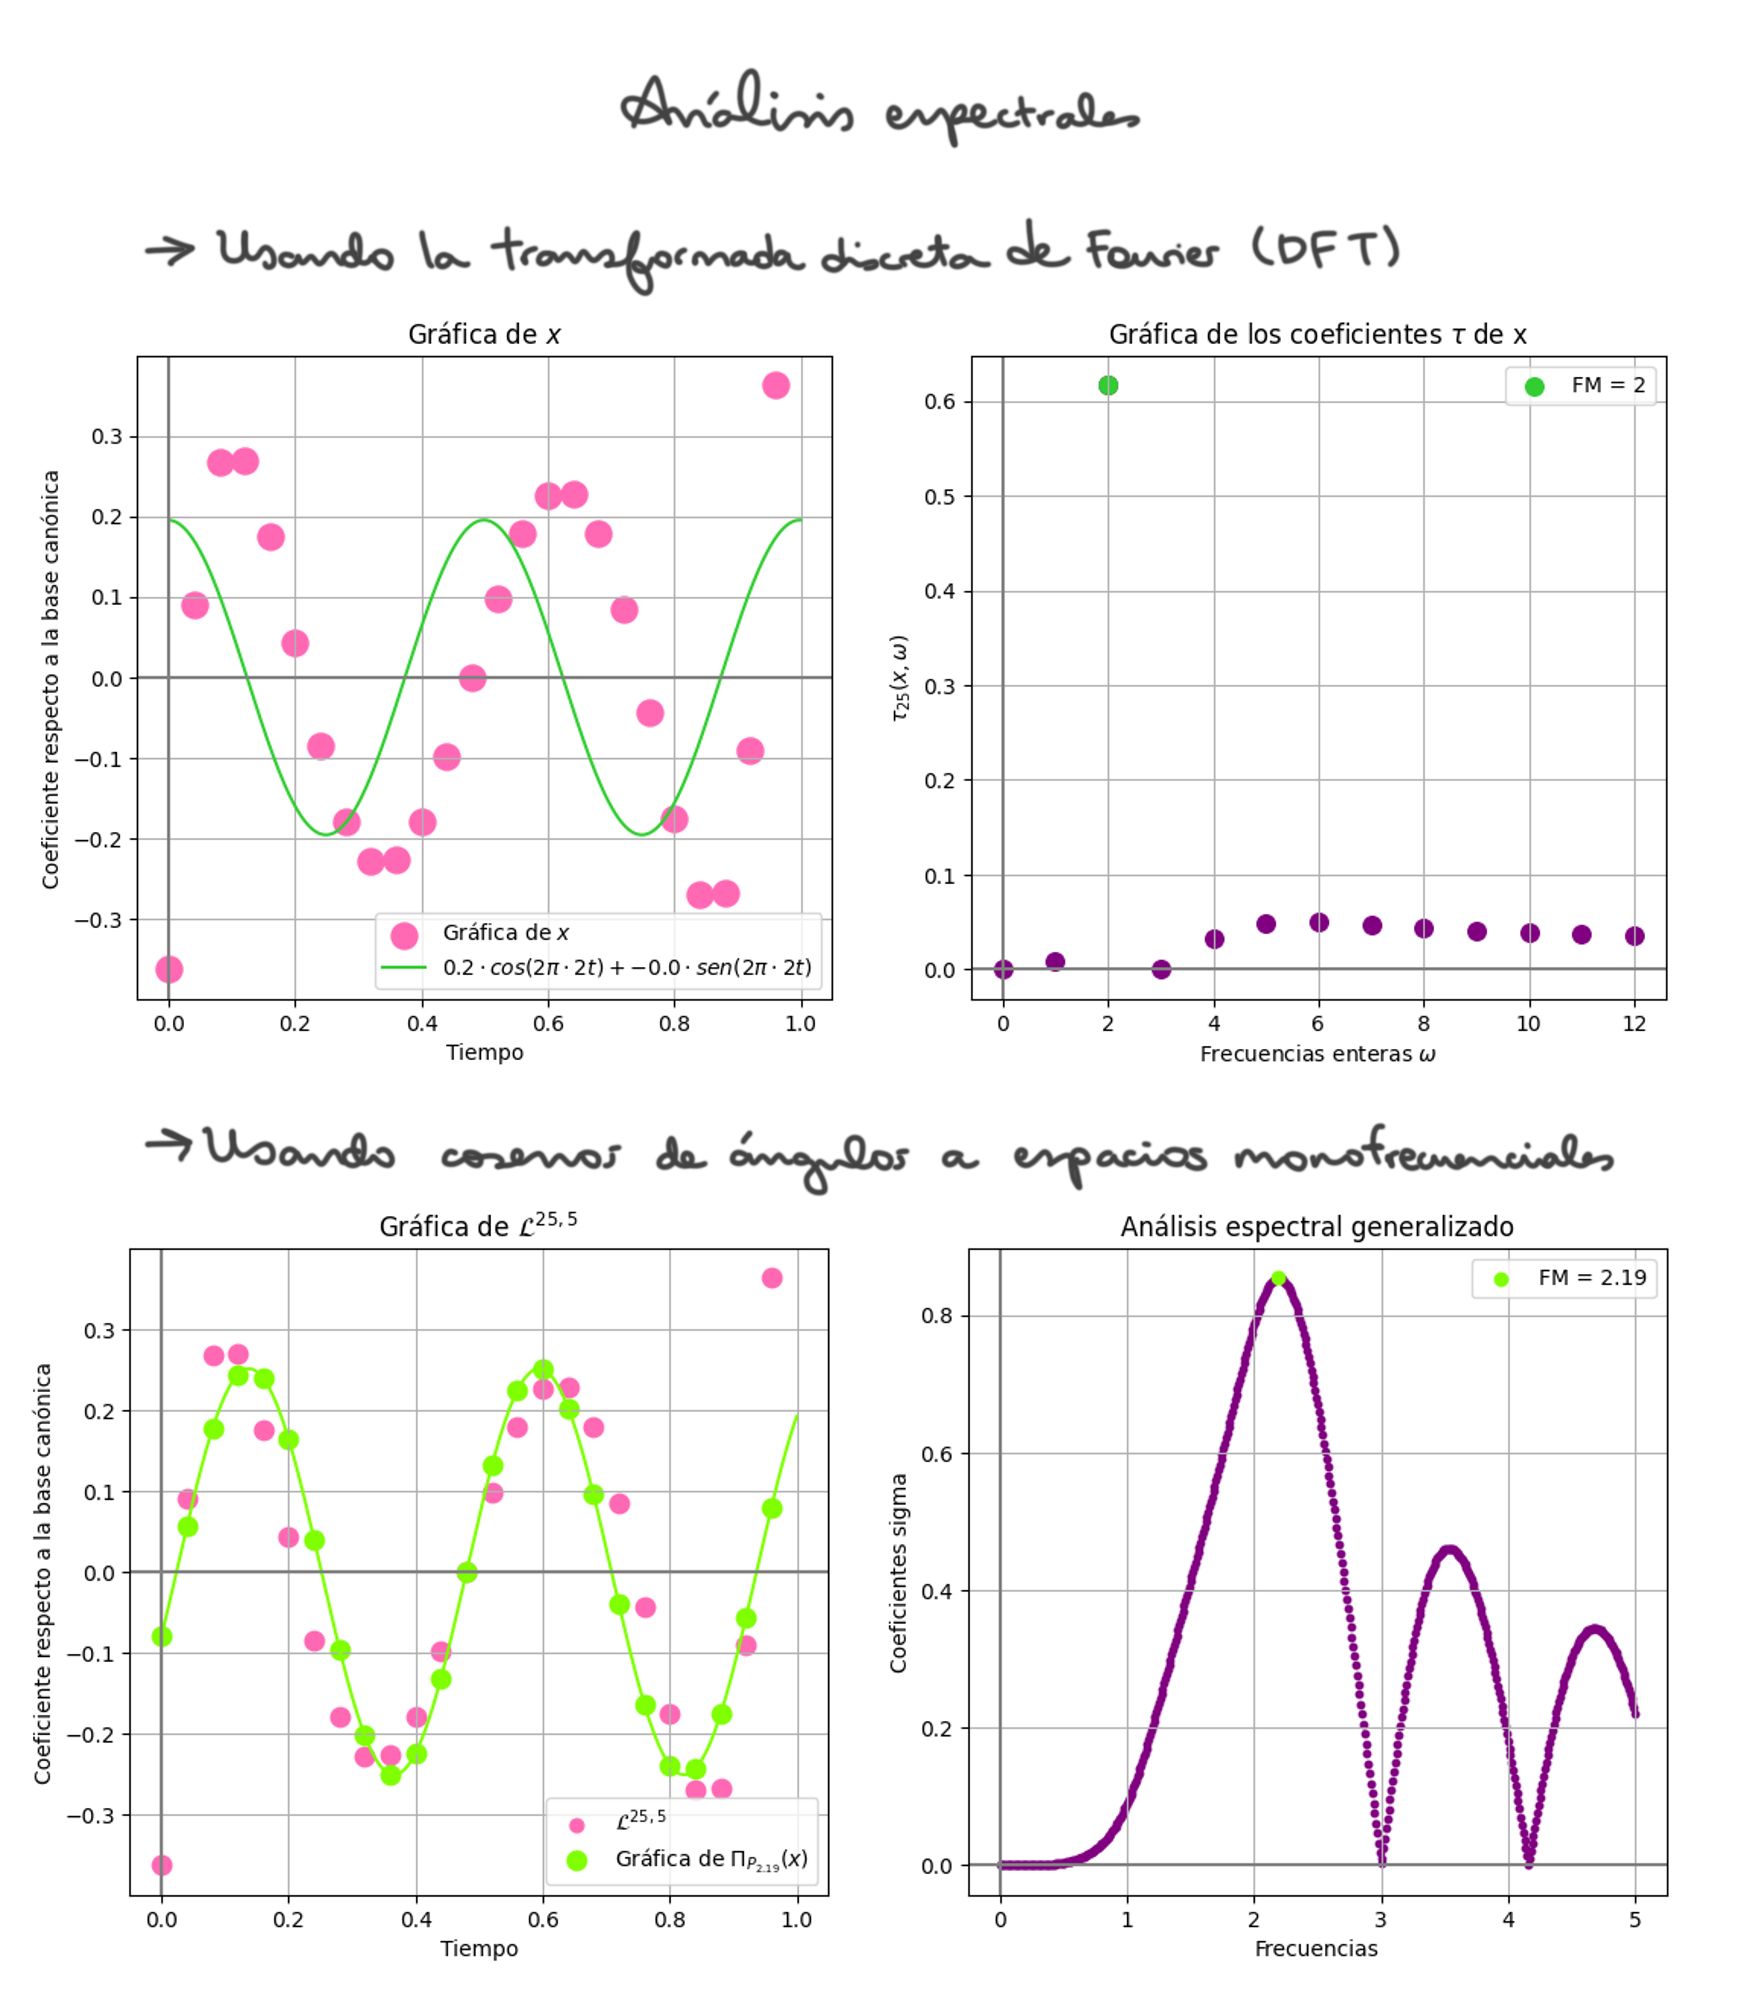
\includegraphics[scale = 1]{ejemplo_analisisEspectrales} 
\end{figure}	

\section{Lista de preguntas a responder usando los resultados numéricos}

\begin{notacion}
Dados los espectros cero y uno de $\cali{L}^{n,k}$, si
$FM_{i}$ 
(para $i=0,1$)
es la frecuencia $\omega$ en la que el espectro 
$i$ alcanza su punto máximo.
\TODO{cambia esto en los cpódgios}
\end{notacion}


Enlistamos las preguntas que nos interesa considerar
(formuladas de manera general, pero que comprobaremos o refutaremos
numéricamente para dimensiones hasta $n=70$, pues para dimensiones
más grandes los errores computacionales son demasiado grandes
como para obtener conclusiones fiables, \TODO{revisa lo que tiene que
decir al respecto el libro de data science!}).

Vamos a responder estas preguntas con gráficas!

La primera pregunta es una reformulación de la 
hipótesis \ref{ref: hipotesis}. Hacemos dos preguntas
más para afinar.

\begin{itemize}
\item \textbf{Pregunta 1}: 
Para cualesquiera $n \geq 2$ y $0 \leq k \leq n-1$,
¿ocurre que las frecuencias máximas
$FM_{0}$ y $FM_{1}$ son cercanas a $\frac{k}{2}$?

\begin{figure}[H]
	\sidecaption{
	\TODO{Voy a responder esta con algunas imágenes de espectros como esta.}
	\label{fig: ejemplo_pregunta1}
	}
	\centering
	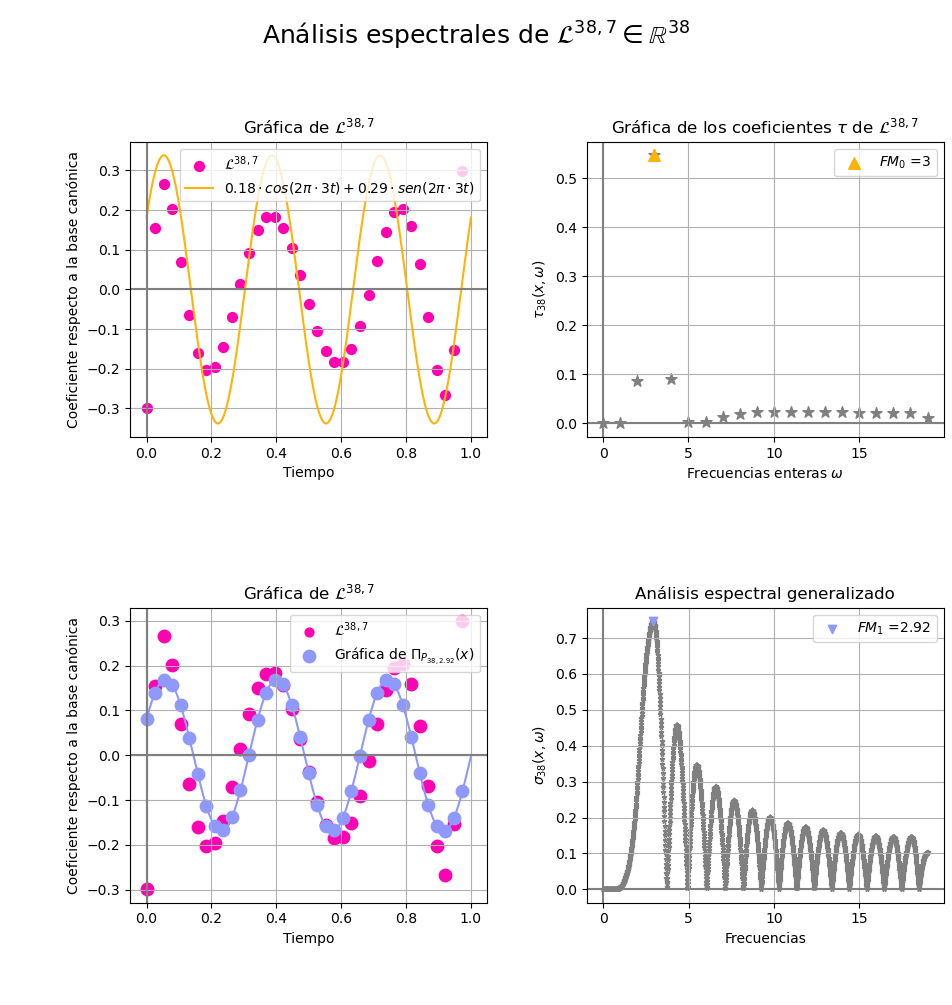
\includegraphics[scale = 0.5]{./estudios_espectrales/ejemplo_pregunta1} 
\end{figure}	

\item \textbf{Pregunta 2}: ¿En efecto dependen $FM_{0}$ y $FM_{1}$ sólo
de $k$ y no de $n$?

\begin{figure}[H]
	\sidecaption{
	\TODO{Voy a responder esta con algunas imágenes de espectros como esta.}
	\label{fig: ejemplo_pregunta2}
	}
	\centering
	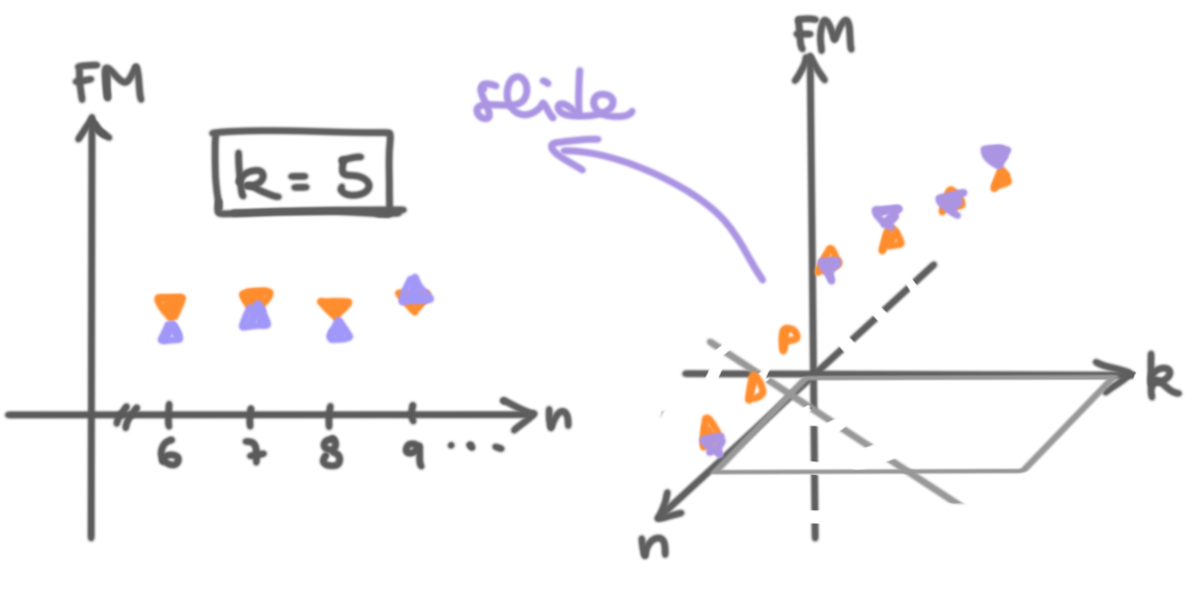
\includegraphics[scale = 1]{./estudios_espectrales/ejemplo_pregunta2} 
\end{figure}	

\item \textbf{Pregunta 3}: ¿Los parámetros $(m,b)$ de pendiente y ordenada al 
origen de las rectas de mínimos cuadrados (RMC) de las gráficas 
de FM para un $n$ fijo son parecidos? ¿En dónde se concentran?
\TODO{reformula mejor.}
\begin{figure}[H]
	\sidecaption{
	\TODO{Voy a responder esta con algunas imágenes de espectros como esta.}
	\label{fig: ejemplo_pregunta3}
	}
	\centering
	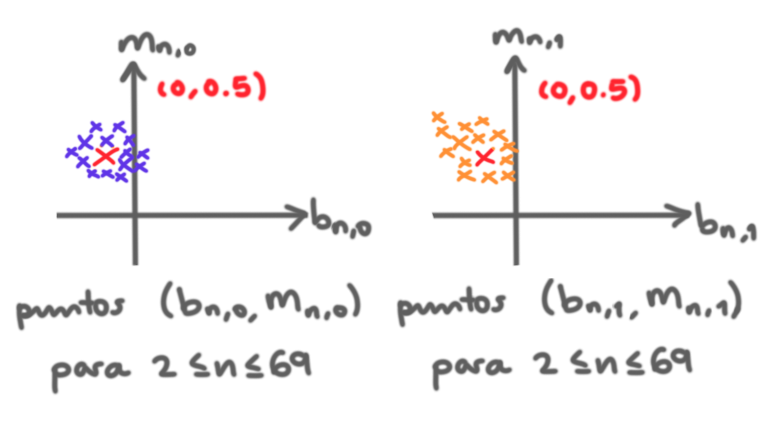
\includegraphics[scale = 1]{./estudios_espectrales/ejemplo_pregunta3} 
\end{figure}	
\end{itemize}

Note que las preguntas 2 y 3 son más bien globales
(y las respondo numéricamente con los datos calculados en 
la función \texttt{analisis$\_$espectralPDL$\_$global}).